\documentclass[12pt,a4paper,titlepage]{article}
\usepackage[a4paper]{geometry}
\usepackage[utf8]{inputenc}
\usepackage[english]{babel}
\usepackage{lipsum}
\usepackage{graphicx}
\graphicspath{ {images/} }
\usepackage[export]{adjustbox}

\usepackage{amsmath, amssymb, amsfonts, amsthm, fouriernc, mathtools}
% mathtools for: Aboxed (put box on last equation in align envirenment)
\usepackage{microtype} %improves the spacing between words and letters

\usepackage{epsfig}
\usepackage{epstopdf}


%%%%%%%%%%%%%%%%%%%%%%%%%%%%%%%%%%%%%%%%%%%%%%%%%%
%% COLOR DEFINITIONS
%%%%%%%%%%%%%%%%%%%%%%%%%%%%%%%%%%%%%%%%%%%%%%%%%%
\usepackage[svgnames]{xcolor} % Enabling mixing colors and color's call by 'svgnames'
%%%%%%%%%%%%%%%%%%%%%%%%%%%%%%%%%%%%%%%%%%%%%%%%%%
\definecolor{MyColor1}{rgb}{0.2,0.4,0.6} %mix personal color
\newcommand{\textb}{\color{Black} \usefont{OT1}{lmss}{m}{n}}
\newcommand{\blue}{\color{MyColor1} \usefont{OT1}{lmss}{m}{n}}
\newcommand{\blueb}{\color{MyColor1} \usefont{OT1}{lmss}{b}{n}}
\newcommand{\red}{\color{LightCoral} \usefont{OT1}{lmss}{m}{n}}
\newcommand{\green}{\color{Turquoise} \usefont{OT1}{lmss}{m}{n}}
%%%%%%%%%%%%%%%%%%%%%%%%%%%%%%%%%%%%%%%%%%%%%%%%%%




%%%%%%%%%%%%%%%%%%%%%%%%%%%%%%%%%%%%%%%%%%%%%%%%%%
%% FONTS AND COLORS
%%%%%%%%%%%%%%%%%%%%%%%%%%%%%%%%%%%%%%%%%%%%%%%%%%
%    SECTIONS
%%%%%%%%%%%%%%%%%%%%%%%%%%%%%%%%%%%%%%%%%%%%%%%%%%
\usepackage{titlesec}
\usepackage{sectsty}
%%%%%%%%%%%%%%%%%%%%%%%%
%set section/subsections HEADINGS font and color
\sectionfont{\color{MyColor1}}  % sets colour of sections
\subsectionfont{\color{MyColor1}}  % sets colour of sections

%set section enumerator to arabic number (see footnotes markings alternatives)
\renewcommand\thesection{\arabic{section}.} %define sections numbering
\renewcommand\thesubsection{\thesection\arabic{subsection}} %subsec.num.

%define new section style
\newcommand{\mysection}{
\titleformat{\section} [runin] {\usefont{OT1}{lmss}{b}{n}\color{MyColor1}} 
{\thesection} {3pt} {} } 

%%%%%%%%%%%%%%%%%%%%%%%%%%%%%%%%%%%%%%%%%%%%%%%%%%
%		CAPTIONS
%%%%%%%%%%%%%%%%%%%%%%%%%%%%%%%%%%%%%%%%%%%%%%%%%%
\usepackage{caption}
\usepackage{subcaption}
%%%%%%%%%%%%%%%%%%%%%%%%
\captionsetup[figure]{labelfont={color=Turquoise}}

%%%%%%%%%%%%%%%%%%%%%%%%%%%%%%%%%%%%%%%%%%%%%%%%%%
%		!!!EQUATION (ARRAY) --> USING ALIGN INSTEAD
%%%%%%%%%%%%%%%%%%%%%%%%%%%%%%%%%%%%%%%%%%%%%%%%%%
%using amsmath package to redefine eq. numeration (1.1, 1.2, ...) 
%%%%%%%%%%%%%%%%%%%%%%%%
\renewcommand{\theequation}{\thesection\arabic{equation}}

%set box background to grey in align environment 
\usepackage{etoolbox}% http://ctan.org/pkg/etoolbox
\makeatletter
\patchcmd{\@Aboxed}{\boxed{#1#2}}{\colorbox{black!15}{$#1#2$}}{}{}%
\patchcmd{\@boxed}{\boxed{#1#2}}{\colorbox{black!15}{$#1#2$}}{}{}%
\makeatother
%%%%%%%%%%%%%%%%%%%%%%%%%%%%%%%%%%%%%%%%%%%%%%%%%%




%%%%%%%%%%%%%%%%%%%%%%%%%%%%%%%%%%%%%%%%%%%%%%%%%%
%% DESIGN CIRCUITS
%%%%%%%%%%%%%%%%%%%%%%%%%%%%%%%%%%%%%%%%%%%%%%%%%%
\usepackage[siunitx, american, smartlabels, cute inductors, europeanvoltages]{circuitikz}
%%%%%%%%%%%%%%%%%%%%%%%%%%%%%%%%%%%%%%%%%%%%%%%%%%



\makeatletter
\let\reftagform@=\tagform@
\def\tagform@#1{\maketag@@@{(\ignorespaces\textcolor{red}{#1}\unskip\@@italiccorr)}}
\renewcommand{\eqref}[1]{\textup{\reftagform@{\ref{#1}}}}
\makeatother
\usepackage{hyperref}
\hypersetup{colorlinks=true}

%%%%%%%%%%%%%%%%%%%%%%%%%%%%%%%%%%%%%%%%%%%%%%%%%%
%% PREPARE TITLE
%%%%%%%%%%%%%%%%%%%%%%%%%%%%%%%%%%%%%%%%%%%%%%%%%%
\title{\blue Data Mining \\
\blueb Assignment Solution $2$}
\author{Vivek Patani}
\date{\today}
%%%%%%%%%%%%%%%%%%%%%%%%%%%%%%%%%%%%%%%%%%%%%%%%%%



\begin{document}
\maketitle
\textit{Please read readme.md for code execution directions, I have tried to maintain a generic structure for each question in coding terms.}
\section{Question 1 Solution}{Download data set Iris and answer the following questions:
}
{%
\subsection{Section 1}{ Calculate the average value and standard deviation for each of the four features.\\~\\
\centerline{Average for Petal Width: 1.2}~\\
\centerline{Variance for Petal Width: 0.58}~\\
\centerline{Standard Deviation for Petal Width: 0.762}~\\~\\
\centerline{Average for Petal Length: 3.76}~\\
\centerline{Variance for Petal Length: 3.09}~\\
\centerline{Standard Deviation for Petal Length: 1.758}~\\~\\
\centerline{Average for Sepal Length: 5.84}~\\
\centerline{Variance for Sepal Length: 0.68}~\\
\centerline{Standard Deviation for Sepal Length: 0.82}~\\~\\
\centerline{Average for Sepal Width: 3.05}~\\
\centerline{Variance for Sepal Width: 0.19}\\
\centerline{Standard Deviation for Sepal Width: 0.436}~\\~\\

\centerline{\textbf{Code Located in q1/q1.py}}
%%% END UBSECTION 1 %%%%%%%%%%%%%%%%%%%%%%%%%%%%%%%%%%%%%%
\subsection{Section 2}{
~\\
\centerline{Repeat the previous step but separately for each type of flower.}\\~\\
\centerline{Average for Sepal Width \& Iris Setosa: 3.42}\\
\centerline{Variance for Sepal Width \& Iris Setosa: 0.14}~\\
\centerline{Standard Deviation for Sepal Width \& Iris Setosa: 0.37416573867739417}~\\~\\
\centerline{Average for Sepal Length \& Iris Setosa: 5.01}~\\
\centerline{Variance for Sepal Length \& Iris Setosa: 0.12}~\\
\centerline{Standard Deviation for Sepal Length \& Iris Setosa: 0.34641016151377546}~\\~\\
\centerline{Average for Petal Width \& Iris Setosa: 0.24}~\\
\centerline{Variance for Petal Width \& Iris Setosa: 0.01}~\\
\centerline{Standard Deviation for Petal Width \& Iris Setosa: 0.1}~\\~\\
\centerline{Average for Petal Length \& Iris Setosa: 1.46}~\\
\centerline{Variance for Petal Length \& Iris Setosa: 0.03}~\\
\centerline{Standard Deviation for Petal Length \& Iris Setosa: 0.17320508075688773}~\\~\\
\centerline{Average for Sepal Width \& Iris Versicolor: 2.77}~\\
\centerline{Variance for Sepal Width \& Iris Versicolor: 0.1}~\\
\centerline{Standard Deviation for Sepal Width \& Iris Versicolor: 0.31622776601683794}~\\~\\
\centerline{Average for Sepal Length \& Iris Versicolor: 5.94}~\\
\centerline{Variance for Sepal Length \& Iris Versicolor: 0.26}~\\
\centerline{Standard Deviation for Sepal Length \& Iris Versicolor: 0.5099019513592785}~\\~\\
\centerline{Average for Petal Width \& Iris Versicolor: 1.33}~\\
\centerline{Variance for Petal Width \& Iris Versicolor: 0.04}~\\
\centerline{Standard Deviation for Petal Width \& Iris Versicolor: 0.2}~\\~\\
\centerline{Average for Petal Length \& Iris Versicolor: 4.26}~\\
\centerline{Variance for Petal Length \& Iris Versicolor: 0.22}~\\
\centerline{Standard Deviation for Petal Length \& Iris Versicolor: 0.469041575982343}~\\~\\
\centerline{Average for Sepal Width \& Iris Virginica: 2.97}~\\
\centerline{Variance for Sepal Width \& Iris Virginica: 0.1}~\\
\centerline{Standard Deviation for Sepal Width \& Iris Virginica: 0.31622776601683794}~\\~\\
\centerline{Average for Sepal Length \& Iris Virginica: 6.59}~\\
\centerline{Variance for Sepal Length \& Iris Virginica: 0.4}~\\
\centerline{Standard Deviation for Sepal Length \& Iris Virginica: 0.6324555320336759}~\\~\\
\centerline{Average for Petal Width \& Iris Virginica: 2.03}~\\
\centerline{Variance for Petal Width \& Iris Virginica: 0.07}~\\
\centerline{Standard Deviation for Petal Width \& Iris Virginica: 0.2645751311064591}~\\~\\
\centerline{Average for Petal Length \& Iris Virginica: 5.55}~\\
\centerline{Variance for Petal Length \& Iris Virginica: 0.3}~\\
\centerline{Standard Deviation for Petal Length \& Iris Virginica: 0.5477225575051661}~\\~\\
}\label{sub:sub2}%
%%% END SUBSECTION 2 %%%%%%%%%%%%%%%%%%%%%%%%%%%%%%%%%%%%%
\subsection{Section 3}{
Draw four box plots, one for each feature, such that each figure shows three boxes, one for each type of flower. Properly label your figures and axes in all box plots. Make sure that the box plots look professional and appear in high resolution. Experiment with thickness of lines, font styles/sizes, etc. and describe what you tried and what looked the most professional.\\
\centering
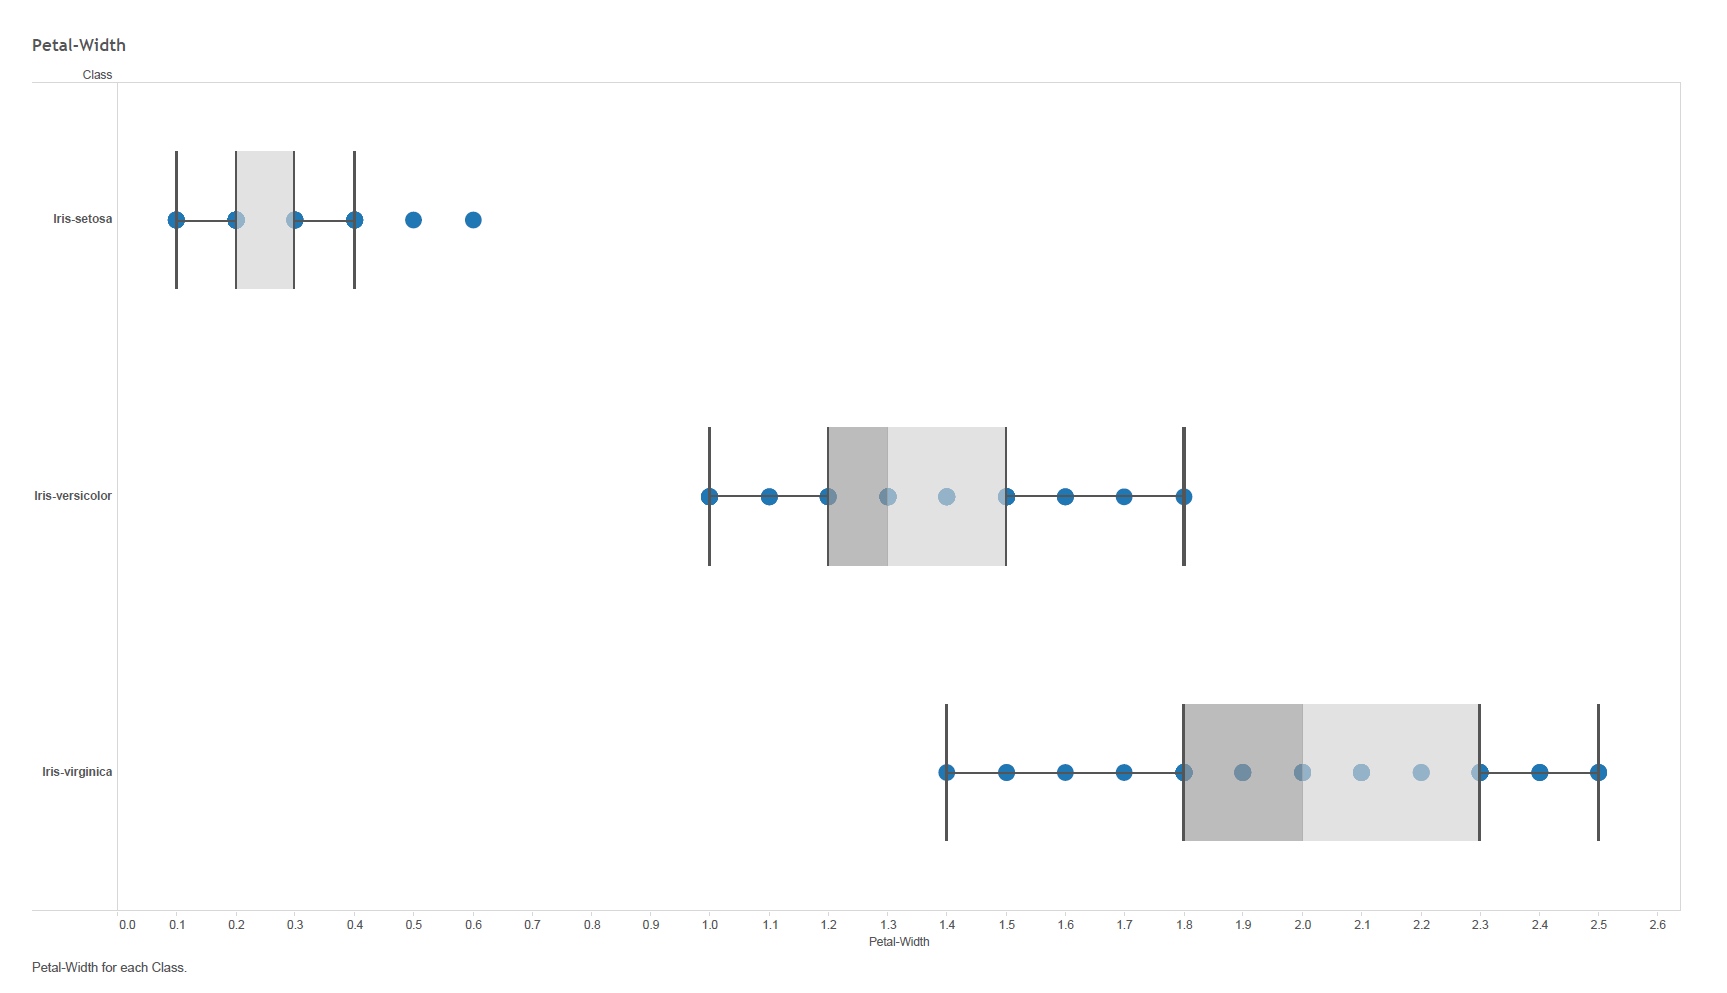
\includegraphics[max size={\textwidth}{\textheight}]{petal-width}\\
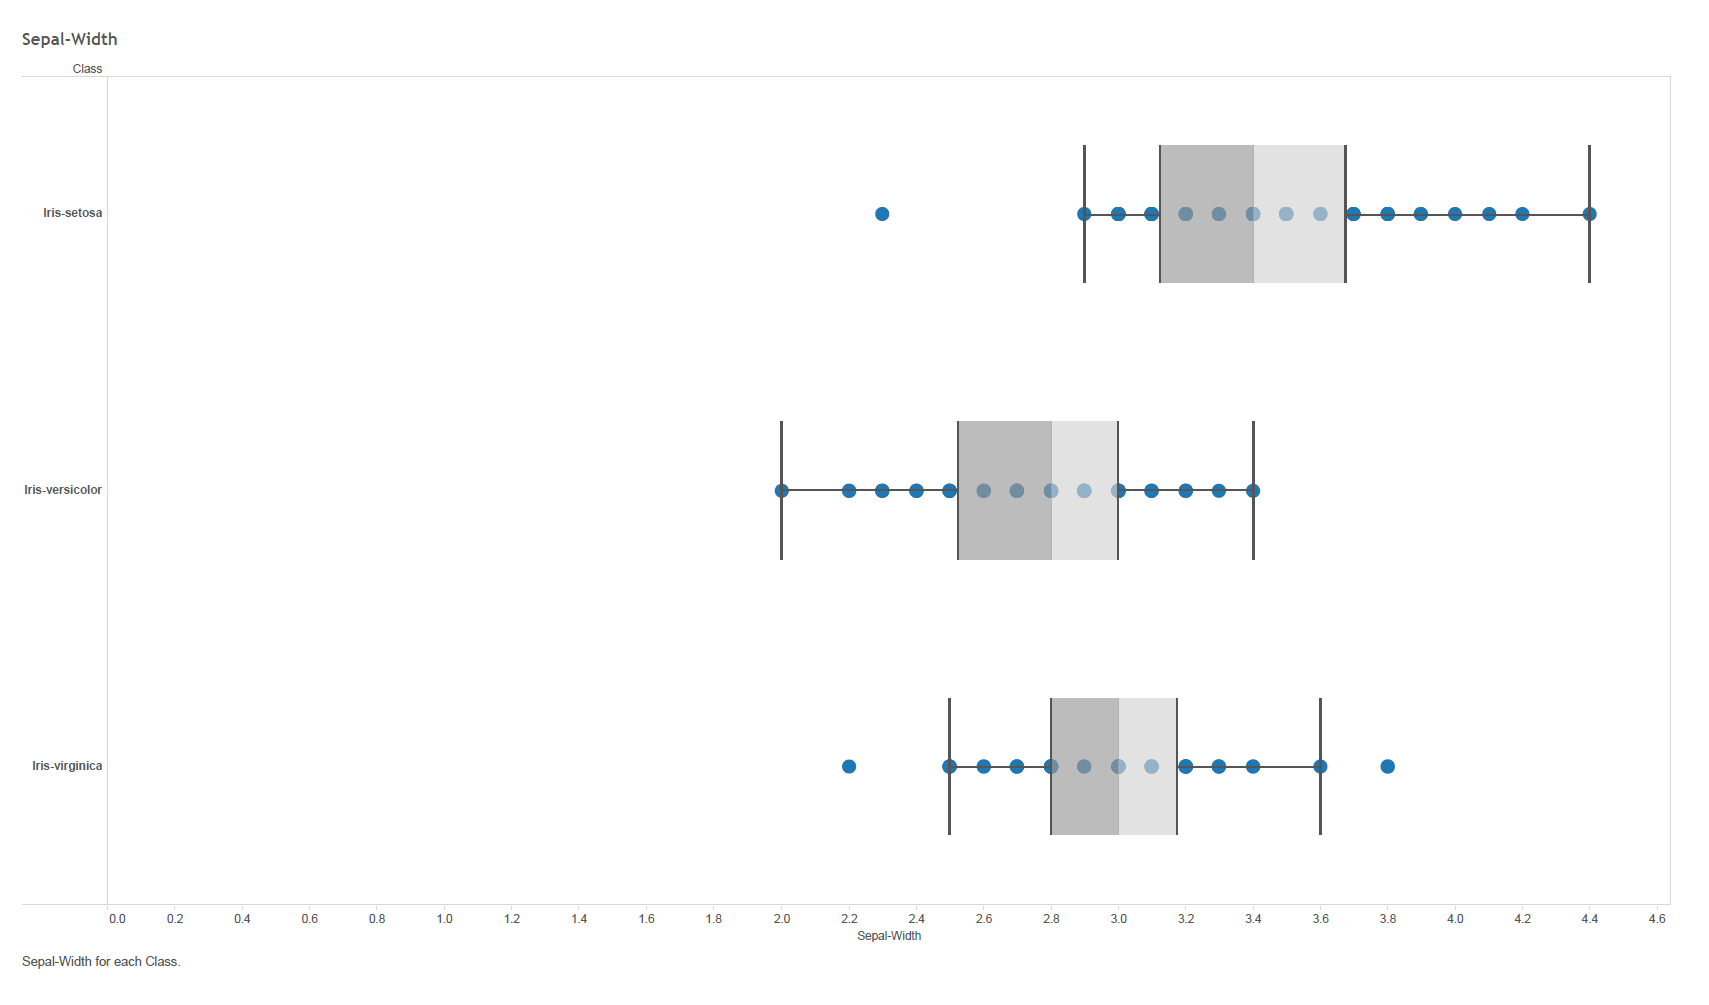
\includegraphics[max size={\textwidth}{\textheight}]{sepal-width}\\
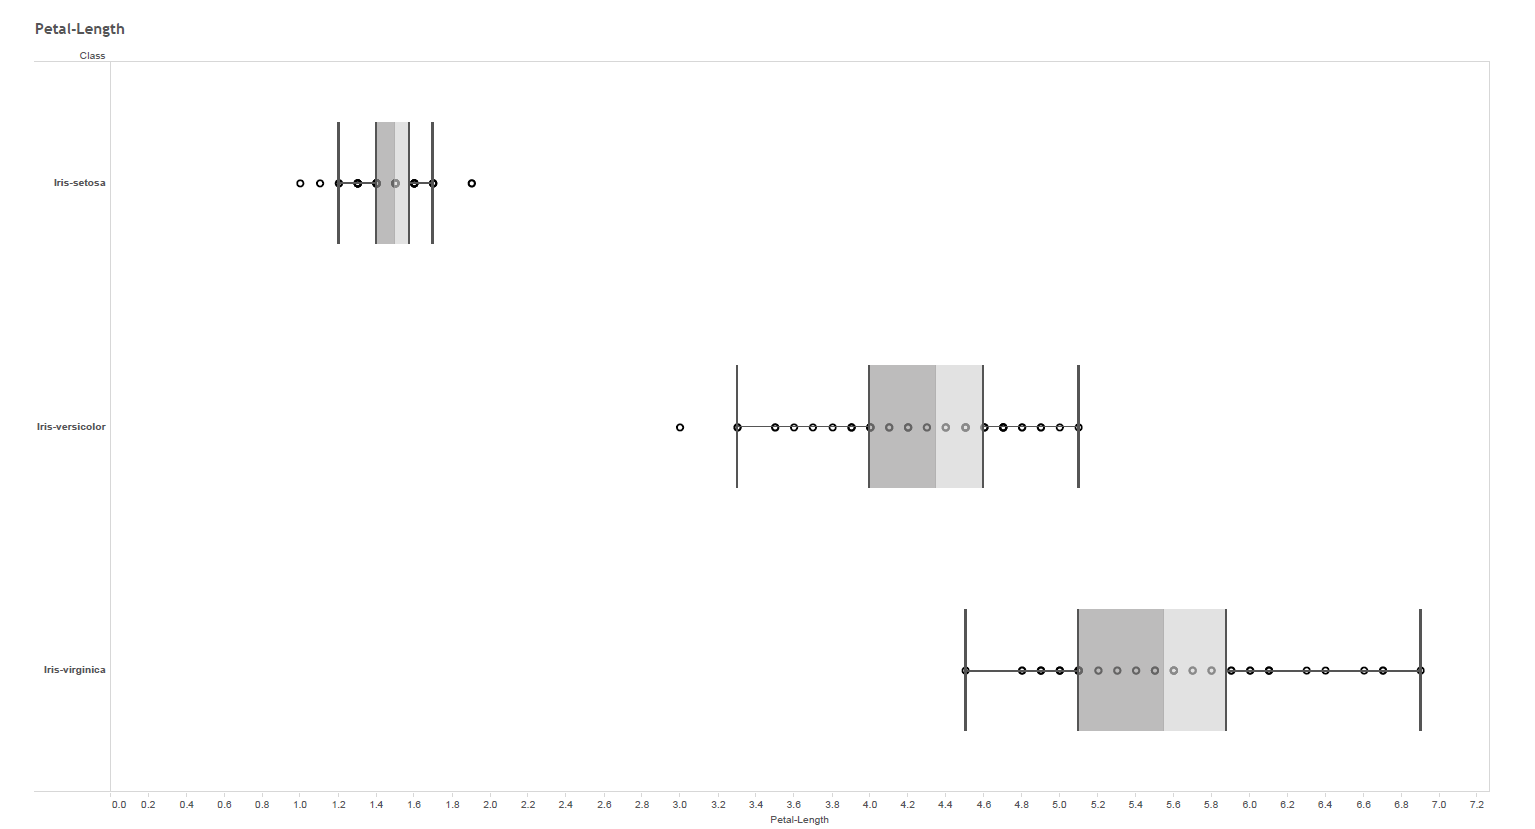
\includegraphics[max size={\textwidth}{\textheight}]{petal-length}\\
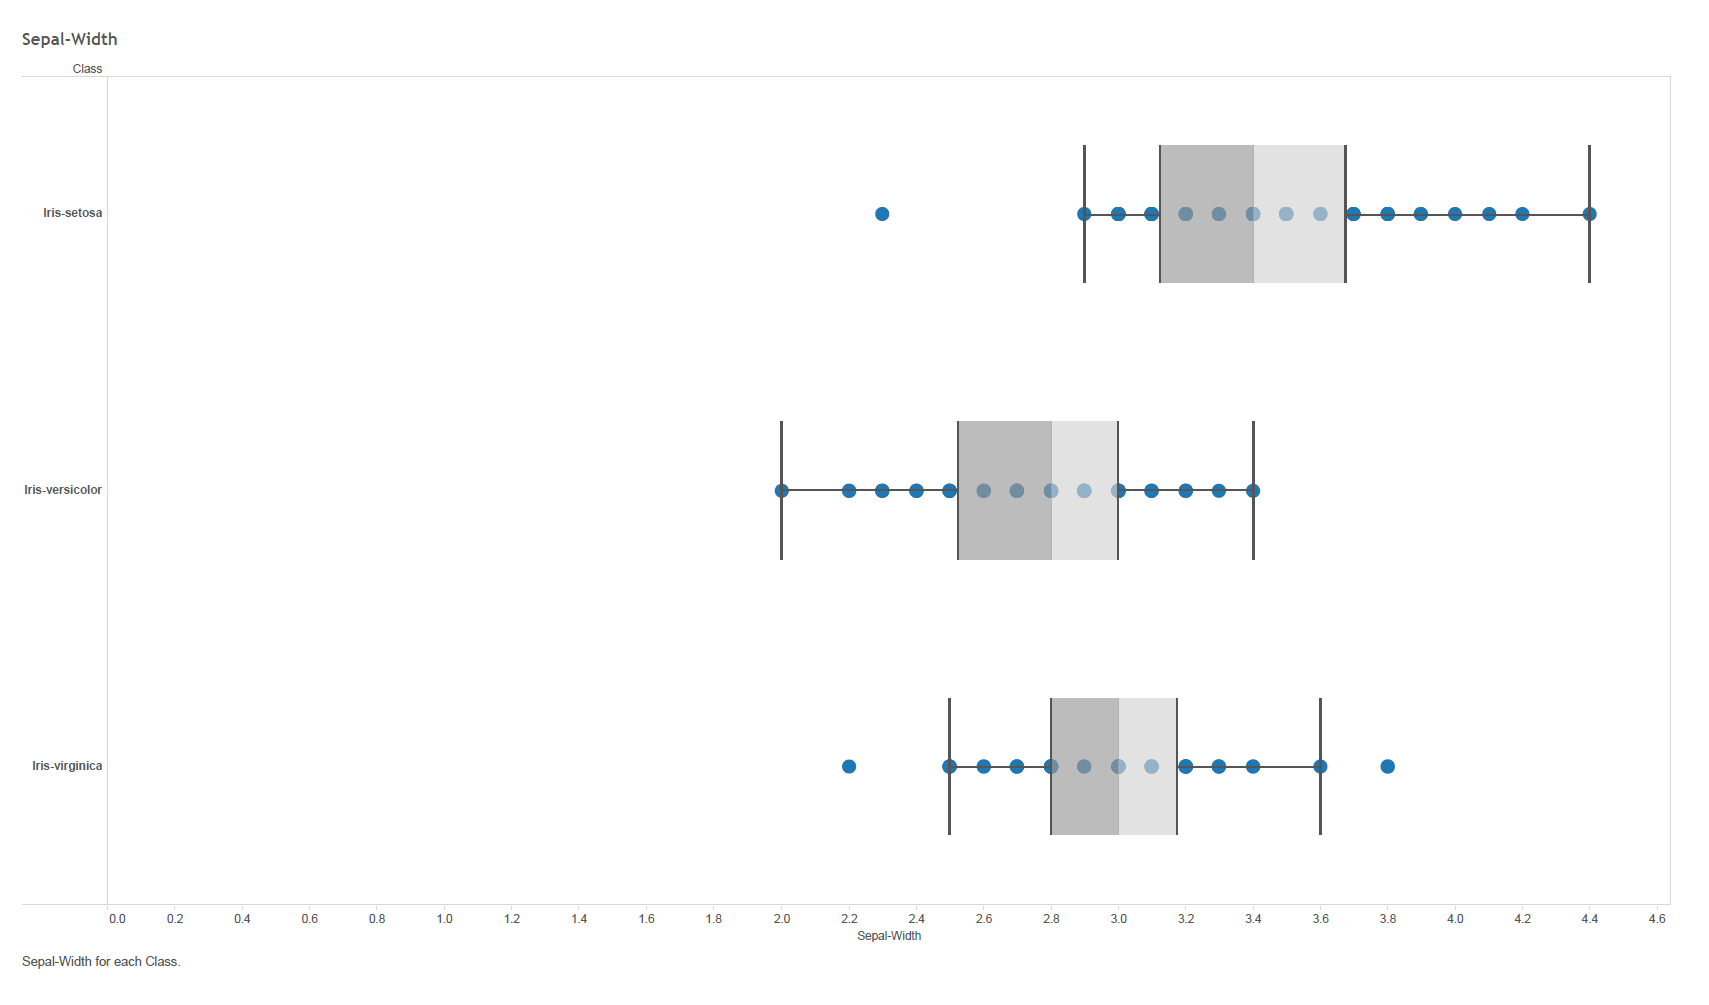
\includegraphics[max size={\textwidth}{\textheight}]{sepal-width}\\
}\label{sub:sub3}
%%% END SUBSECTION 3 %%%%%%%%%%%%%%%%%%%%%%%%%%%%%%%%%%%%%
}
%%% END SECTION 1 %%%%%%%%%%%%%%%%%%%%%%%%%%%%%%%%%%%%%%%



\section{Question 2 Solution}{
Download data set Wine and answer the following questions
\subsection{Section 1}{
Provide pairwise scatter plots for four most correlated and four least correlated pairs of features, using Pearson's correlation coefficient. Label all axes in all your plots and select fonts of appropriate style and size. Experiment with different ways to plot these scatter plots and choose the one most visually appealing and most professionally looking.\\~\\
\centering
The data is preprocessed through a Python Script and R for visualisations. Actually the python script is redundant since everything was done in R later on in R itself because Math Plot lib wasn't working. It was easier through R.
The four most correlated pairs were:\\
1.) Flavanoids - Non Flavanoid Phenols: 0.86\\
2.) Non Flavanoid Phenols - Proline: 0.78\\
3.) Flavanoids - Proline: 0.69\\
4.) Non flavanoid Phenols - Color Intensity: 0.65\\
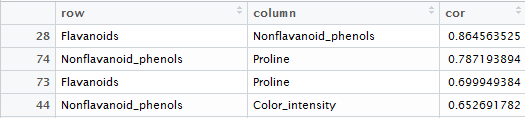
\includegraphics[max size={\textwidth}{\textheight}]{maxcorrelated}\\
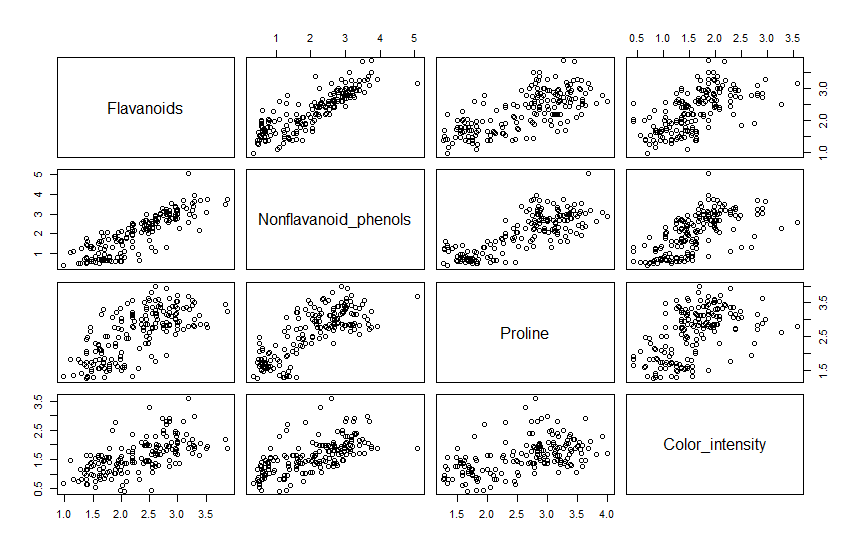
\includegraphics[max size={\textwidth}{\textheight}]{max_corr}\\

The four least correlated pairs were:\\
1.) Alcanility of Ash - Proline: 0.03\\
2.) Alcanility of Ash - Color Intensity: 0.09\\
3.) Color Intensity - Hue: -0.02\\
4.) Magnesium - Hue: 0.18\\
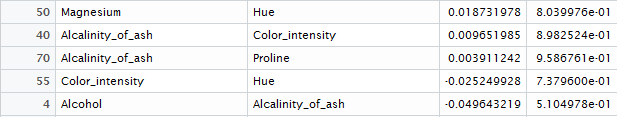
\includegraphics[max size={\textwidth}{\textheight}]{min_corr}
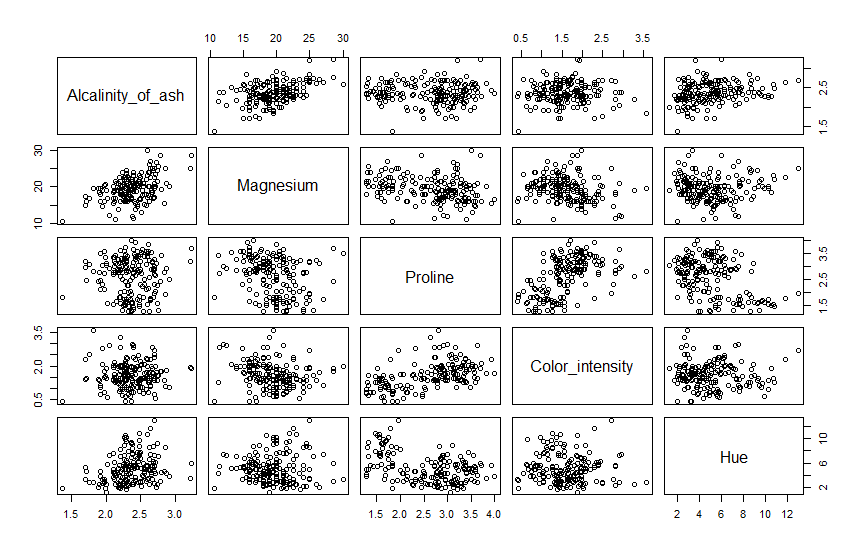
\includegraphics[max size={\textwidth}{\textheight}]{no_corr}\\

\centerline{\textbf{Code in q2/a}}
}

%%% END SUBSECTION 1 %%%%%%%%%%%%%%%%%%%%%%%%%%%%%%%%%%%%%%

\subsection{Section 2}{
Use Euclidean distance to find the closest example to every example available in the data set (exclude the class variable). Calculate the percentage of points whose closest neighbours have the same class label (for data set as a whole and also for each class).\\~\\
The algorithm is straight forward and following a Brute Force method. The algorithm compares the data points to every other points in the set. This is then, checked upon each condition by keeping a count. The count is then incremented checking based on each condition whether if it lies in the same class at all or not. We find the minimum \\~\\
Formula (Overall) = Total Matching / Total No of Computation\\~\\
Formula (Each) = Total Of that Class / Total No of Computation for that class total.\\~\\
\centering{Statistics}~\\
\centerline{Complete Dataset: 76.8 \%}~\\
\centerline{Class 1: 88.1 \%}~\\
\centerline{Class 2: 76 \%}~\\
\centerline{Class 3: 64.5 \%}~\\
\centerline{Code in q2/b-c}~\\

}
%%% END SUBSECTION 2 %%%%%%%%%%%%%%%%%%%%%%%%%%%%%%%%%%%%%%

\subsection{Section 3}{
Repeat the previous step but after the data set is normalized using first 0-1 normalization and then z-score normalization. Investigate the reasons for discrepancy and provide evidence to support every one of your claims. Provide the code you used for normalizing and visualizing the data.\\~\\

\centerline{0 - 1 Normalization}~\\
\[ z_i=\frac{x_i-\min(x)}{\max(x)-\min(x)} \]
}

\begin{verbatim}
#0-1 Normalisation
normalise  <- function(x) {
    final_data1 <- ((x - min(x))/(max(x) -min(x)))
  return (final_data)
  }
\end{verbatim}
\centerline{Statistics}
\centerline{Full Set Accuracy: 95\%}
\centerline{Class 1 Set Accuracy: 100\%}
\centerline{Class 2 Accuracy: 87.8\%}
\centerline{Class 3 Accuracy: 100\%}

\centerline{Z Score Normalization}~\\
\[x^\prime := (x-x_{\min})/(x_{\max} -x_{\min} )\]
\begin{verbatim}
#Z Score Normalisation
z_score<-function(x){
    scale(x)
    final_data <- ((x - mean(x)) / sd(x))
    return (final_data)
  }
}
\end{verbatim}
\centerline{Statistics}
\centerline{Full Set Accuracy: 95\%}
\centerline{Class 1 Set Accuracy: 99.9\%}
\centerline{Class 2 Accuracy: 88.3\%}
\centerline{Class 3 Accuracy: 100\%}
}~\\
The idea of \textbf{Normalization} comes to data mining when we need to actually render the data in a specific range. It is used to make more sense out of the data, say when we have to actually data that is non - linear and to bring them to a linear state to form a relationship is one instance where we can use normalisation. There are a few techniques used for normalisation such min-max norm, 0-1 normalisation, Decimal Scaling etc. The drawback of normalization is that the data comes really close to each other and may sometimes cross boundaries. So if in a dataset where points have a few sparse data points, while normalising they may come really close and would give you an unclean result. Normalisation should be performed only when required.\\~\\
%%% END SUBSECTION 3 %%%%%%%%%%%%%%%%%%%%%%%%%%%%%%%%%%%%%%
%%% END SECTION 2 %%%%%%%%%%%%%%%%%%%%%%%%%%%%%%%%%%%%%%%%



\section{Question 3 Solution}{
Data exploration is often the first step in many data analysis tasks. Visualizing relationships between features as well as between features and the target variable(s), for example, can be exploited to design a good model or to understand why a particular model works. There are many software packages developed to make this step easier. In this question you will experiment with Tableau.
\subsection{Section 1}{
Download and study the Auto MPG data set from the UCI Machine Learning Repository.
Import the data set into Tableau. Create a new feature make (Honda, Toyota, . . . ) that contains the make of the automobile (extract this feature automatically from other features through Tableau) and in a single figure generate box plots of mpg for 10 makes of your choice. Then, for 5 makes of your choice create scatter plots of weight versus mpg. Include all figures in your submission and comment on what you observe.\\~\\

\centering
This is a Box Plot for 10 makes.\\
The data here tells us that Honda gives a good MPG and cars such as Buic, Dodge and Ford provide a wide range of MPG's which tells us that they must be producing a wide range of cars and probably a good amount of models ranging from basic to high end.
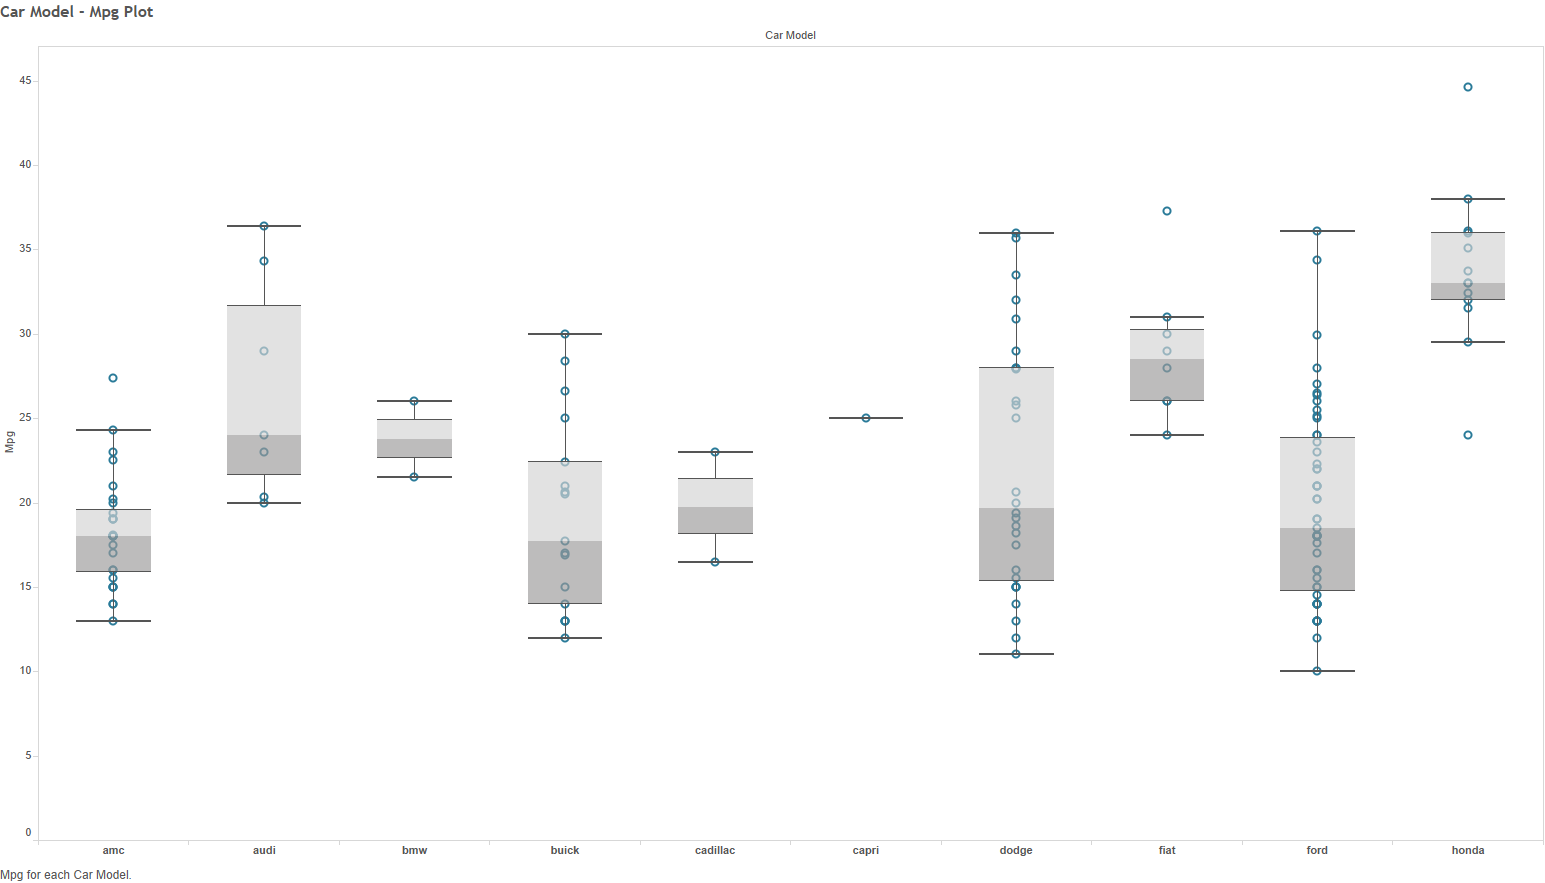
\includegraphics[max size={\textwidth}{\textheight}]{10}\\
This is a Scatter Plot for 5 makes.\\
This plot describes a rather negative correlation between Weight and MPG. This is also true mostly in real life and which is quite a logical thing. The legends display the 5 makes for which we are drawing conclusions.
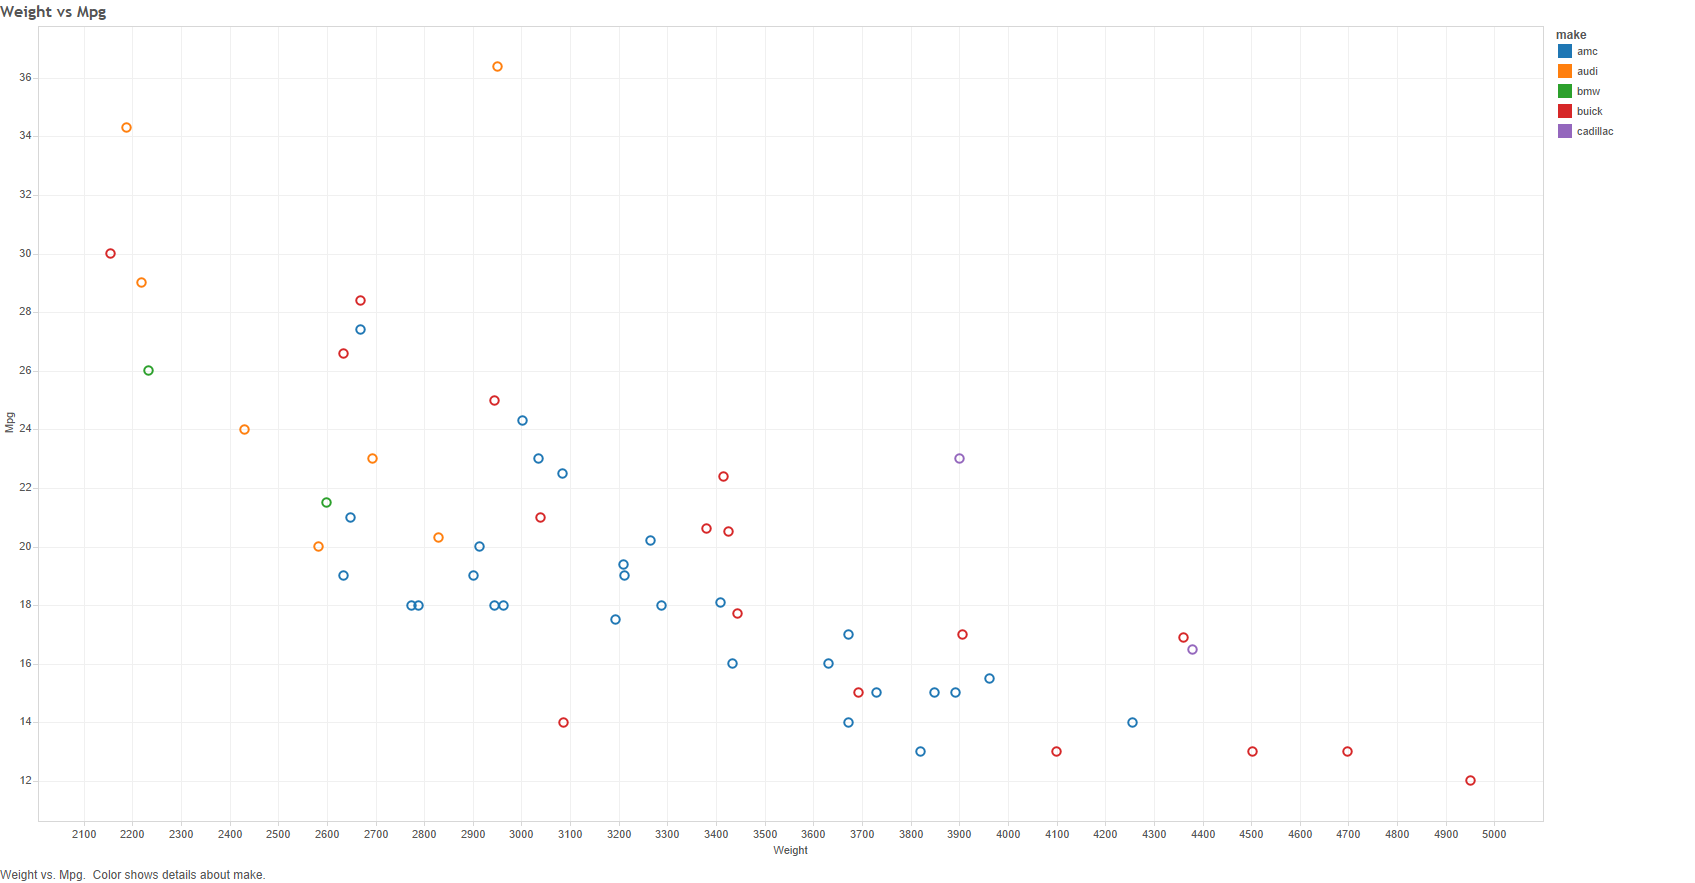
\includegraphics[max size={\textwidth}{\textheight}]{Weightvsmpg}\\

}
%%% END SUBSECTION 1 %%%%%%%%%%%%%%%%%%%%%%%%%%%%%%%%%%%%%%


\subsection{Section 2}{Pick 3 data sets of your choice from UCI Machine Learning Repository. Visualize each the data set in meaningful ways that show hidden patterns. Experiment with colors, size, shapes, filters,groups and sets. Feel free to experiment with other advanced functionalities of Tableau.\\~\\
\centering
The data set used here is the adult dataset from the UCI ML repo.\\
(Link: http://mlr.cs.umass.edu/ml/datasets/Adult)\\
We observe the distribution of sex among specific working classes and a few other filters are applied. We see that while private housing service has more females others are more dominated by males. This tells us that we should encourage more females in the other departments to create equality in each work domain.\\
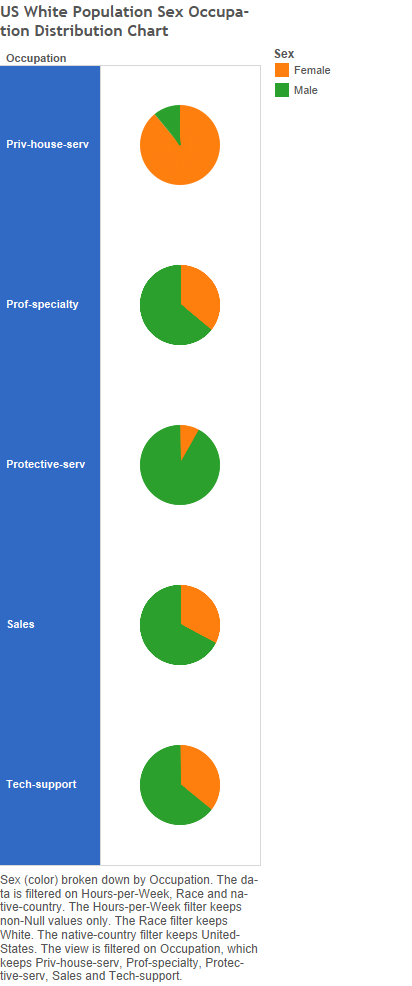
\includegraphics[max size={\textwidth}{\textheight}]{US_Population}\\
This data is the wine dataset taken from UCI ML Repo.\\
(Link: http://archive.ics.uci.edu/ml/datasets/Wine)\\
The PH and density a rather negative correlation among them. But the interesting observation is that most of the values are pretty closely clustered and tells us that the ratio of PH and density is pretty much constant.
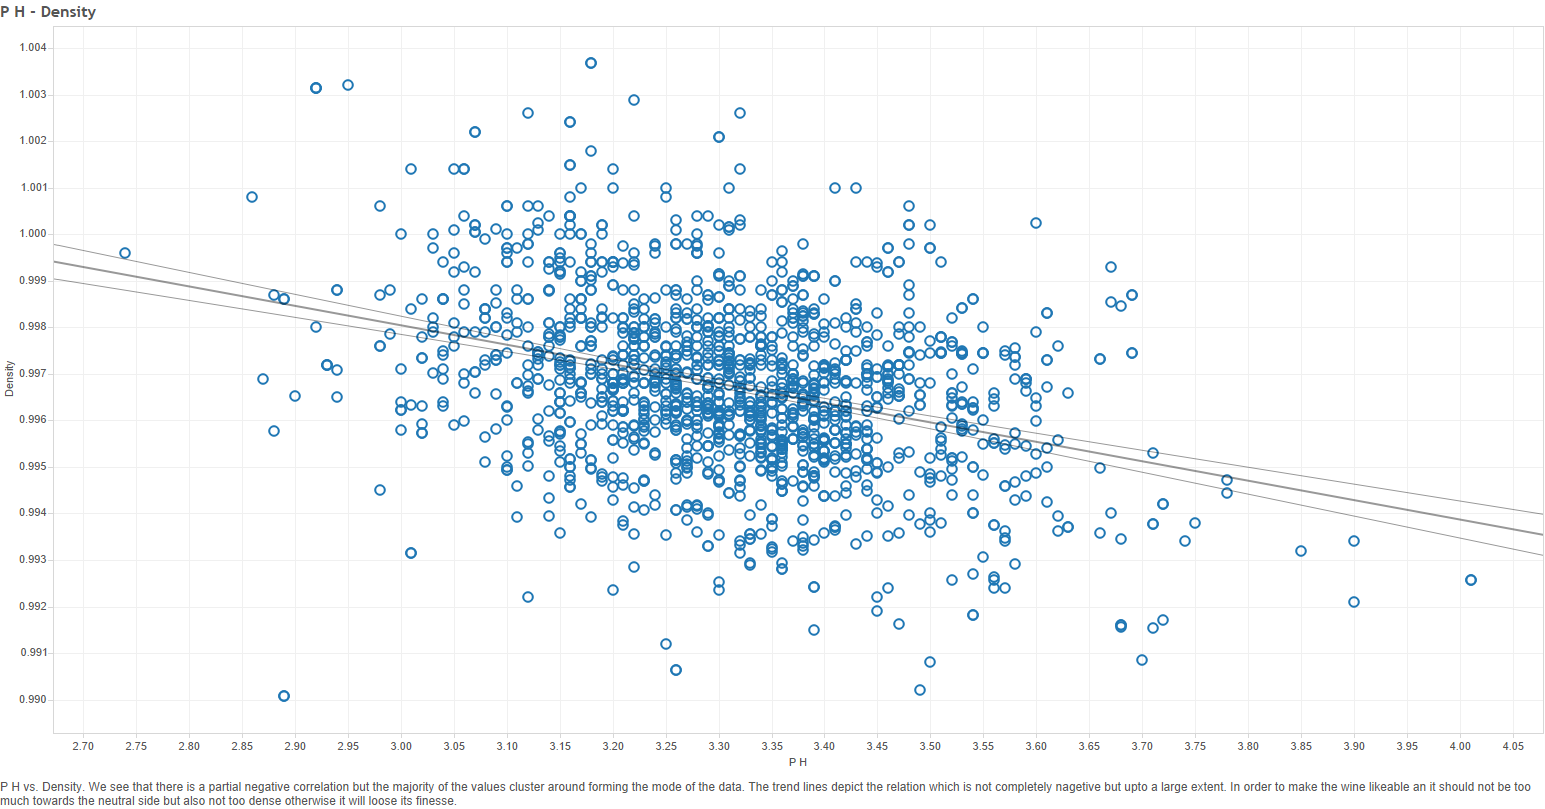
\includegraphics[max size={\textwidth}{\textheight}]{PhvsDensity}\\
This is the Glass ID Dataset\\
(Link:https://archive.ics.uci.edu/ml/datasets/Glass+Identification)\\
The scatter plot tells us that the data is pretty sparse and we can see that there is no correlation between or rather very less amount of correlation. The mean value lies about RI:1.5 and Aluminium Oxide:1.45.
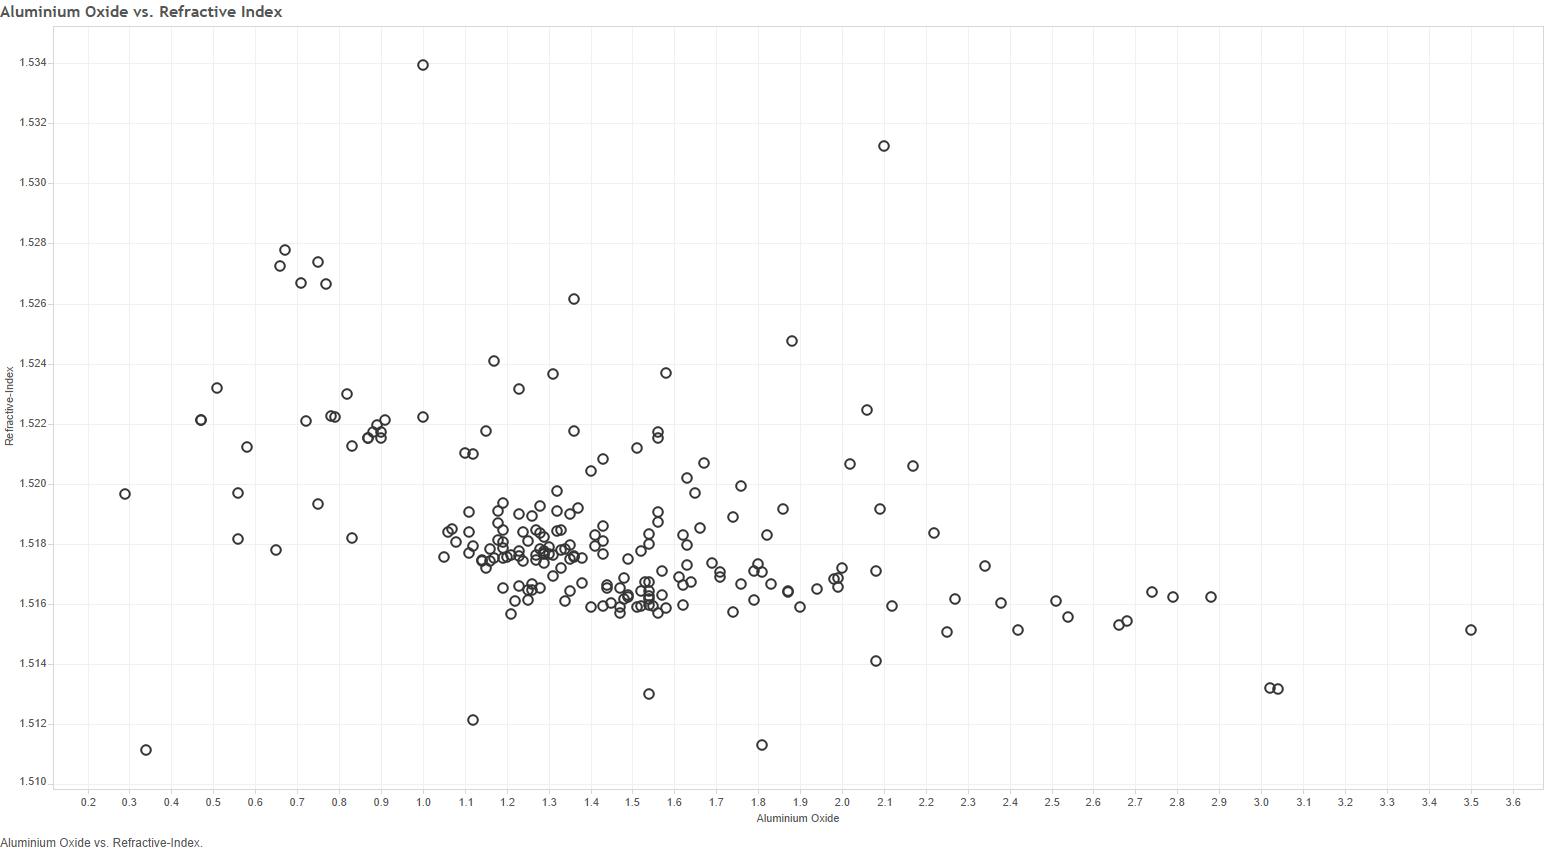
\includegraphics[max size={\textwidth}{\textheight}]{alri}\\
This is the Glass ID Dataset\\
(Link:https://archive.ics.uci.edu/ml/datasets/Glass+Identification)\\
The Graph tells us that the data is pretty correlated and in a positive way, so the relation is that the data is RI increases with increase in the Caclcium Oxide Content and but is limited to a certain extent.\\
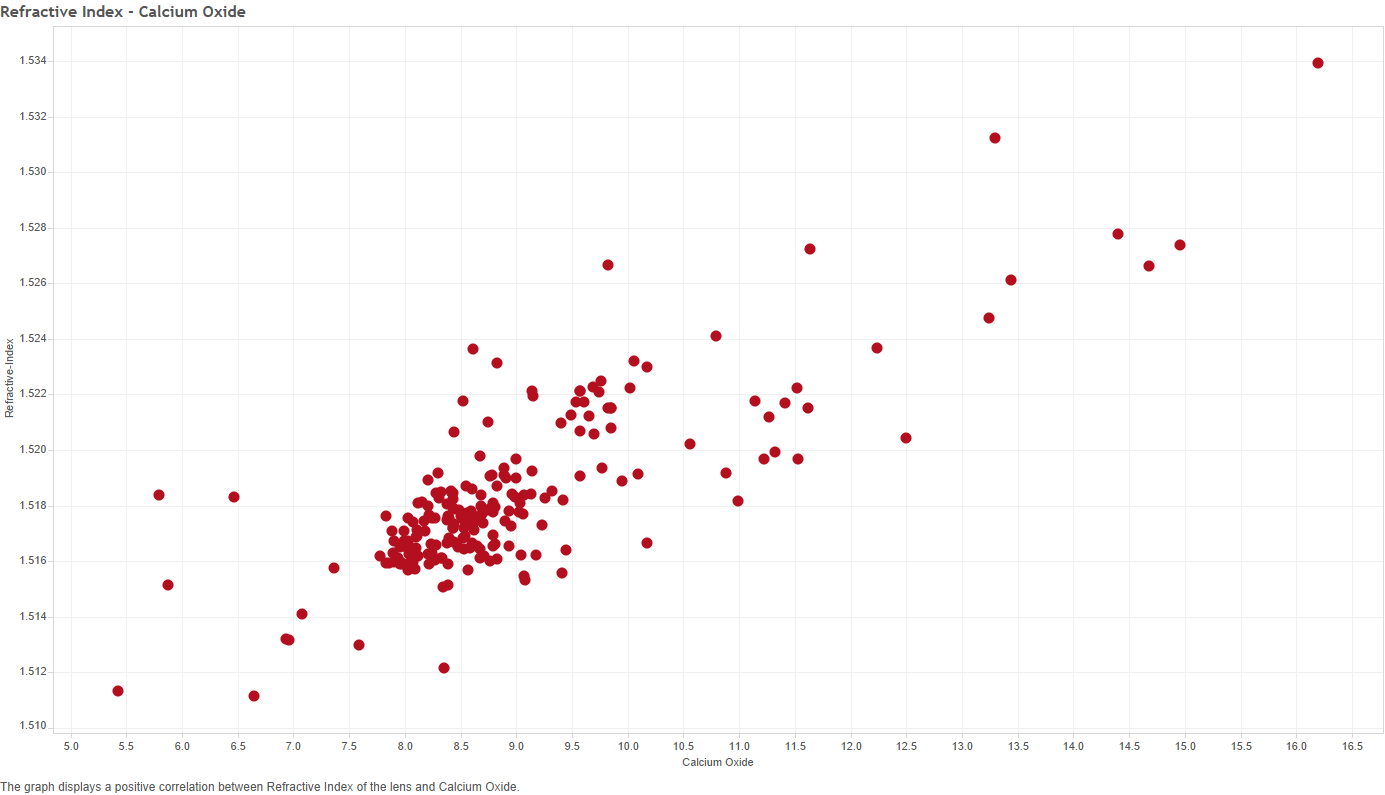
\includegraphics[max size={\textwidth}{\textheight}]{co}\\
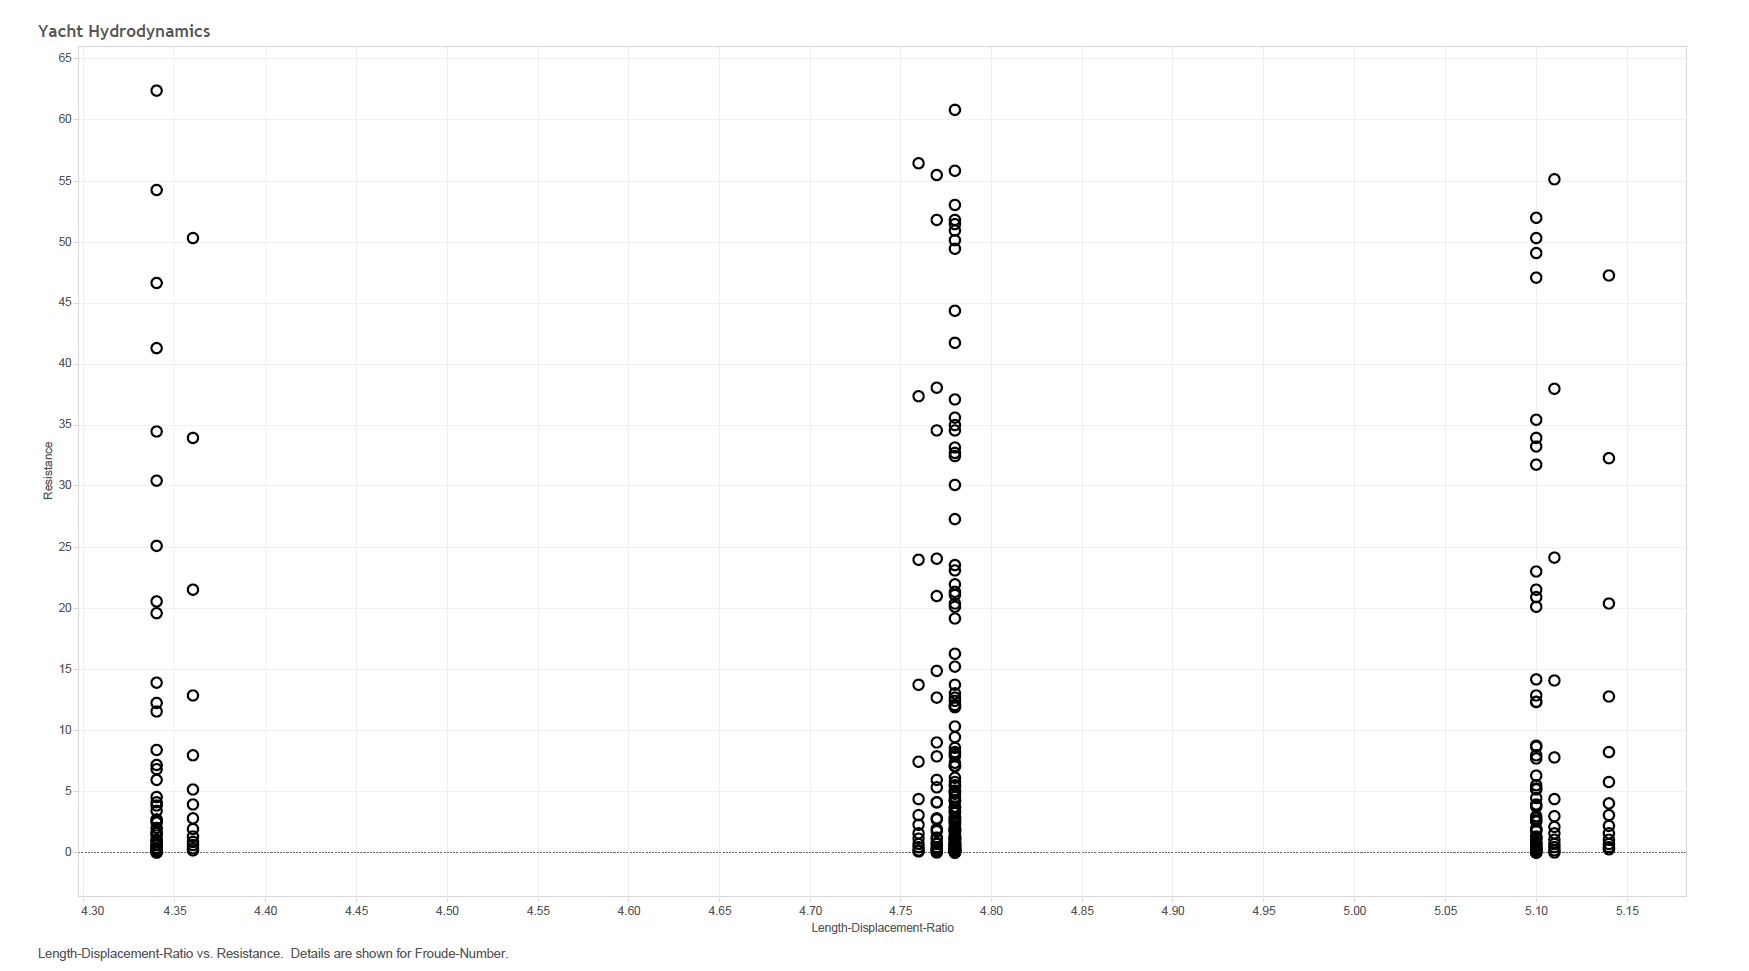
\includegraphics[max size={\textwidth}{\textheight}]{q3b-yacht}\\

}
%%% END SUBSECTION 2 %%%%%%%%%%%%%%%%%%%%%%%%%%%%%%%%%%%%%%

\subsection{Section 3}{ Tell us about your experience with Tableau. What did you learn? What did you like/dislike about Tableau?\\~\\
Good things:\\
1.) The loading of data is pretty easy. Also the support for various datasets is wide.\\
2.) The filter application is great, since it gives you all the unique values to select from all the attribute values. Elimination and Error Handling of Null values is also taken care of.\\
3.) Produces neat and clean visualisations with relevant legends, axis, title and caption.
\\~\\
Bad Things:\\
1.) JSON direct import is not available, need an API. I believe JSON to be well established and well structured to be included.\\
2.) Well it is fairly good for small datasets but takes a lot of while to import large datasets.\\
3.) Data Transformation is fairly limited because of the ability to manipulate.\\
}
%%% END SUBSECTION 4 %%%%%%%%%%%%%%%%%%%%%%%%%%%%%%%%%%%%%%
%%% END SECTION 3 %%%%%%%%%%%%%%%%%%%%%%%%%%%%%%%%%%%%%%%
}
\section{Question 4 Solution}{
\centerline{Implementing classification trees and evaluating their accuracy}
\subsection{Section 1}{Implement the greedy algorithm that learns a classification tree given a data set. Assume that all features are numerical and properly find the best threshold for each split. Use Gini and information gain, as specified by user, to decide on the best attribute to split in every step. Stop growing the tree when all examples in a node belong to the same class or the remaining examples contain identical features.\\~\\

\centerline{Algorithm}~\\
1.) The primary step is to clean up the data by putting the class variable to the right hand side column (making the class the last attribute, since I started with Iris and then have done that for datasets onwards). (code: q4-data formatter.py) - Using pickle to pull and push data since it stores data as is.\\
2.) Defined a class Node (which contains a simple class to store the node structure). (node.py)\\
3.) Then we need to divide the dataset by calculating Entropy or Gini Impurity, based on that attribute we split the data. For initiation we use the 0th attribute. (Code: divide.py and impurity.py)\\
4.) Then we build the tree using the division based on the attribute selection and store everything on the node.(buildtree.py)\\
5.) Print tree is used to generate a tree picture.(printtree.py)\\
6.) There is a main.py script which runs the complete script (This has parts of Qustion 5 running together, script has comments on running the 4th only).\\
References for this: http://kldavenport.com/pure-python-decision-trees/ - This is my basic tutorial what I started off with.\\~\\
}
\subsection{Section 2}{
Implement 10-fold cross-validation to evaluate the accuracy of your algorithm on 10 different data sets from the UCI Machine Learning Repository. Select only those data sets where all features are numerical. In certain cases you can convert categorical features into numerical by encoding them using sparse binary representation. That is, if feature values belong to a set {blue, yellow,red, green}, encode this feature using 4-dimensional binary vectors such that if the feature value is blue, the encoding is (1, 0, 0, 0), if the feature value is yellow, the encoding is (0, 1, 0, 0), etc. You can also transform regression problems from the repository into classification problems by using the mean of the target variable to dichotomize the continuous target into binary class labels\\~\\

1.) The ten folding is done with the help of dividing strata of data using Stratified K folding. Pythons Scikit has a library to do this. Say you have 150 values so it splits 150/K sets of test and train. Our K = 10(genkfolds.py)\\

2.) In this the conversion of categorical attributes is performed to make them numeric. We check in the condition for a numeric (float or int) value or non numeric value.\\

3.) Classification is applied using all test data points generated and then checking for accuracy. The accuracy (accuracy.py) is checked for the number of false and true predictions.\\ Accuracy = Correctly Predicted Instances / Total Predictions made\\~\\

Accuracy for Iris: 99\% on an average.\\
Accuracy for Haberman: 76\% on an average.\\
Accuracy for Wine: 97\% on an average.\\
Accuracy for Banknote: 95\% on an average.\\
Accuracy for Yeast: 54\% on an average.\\
\centering
IRIS\\
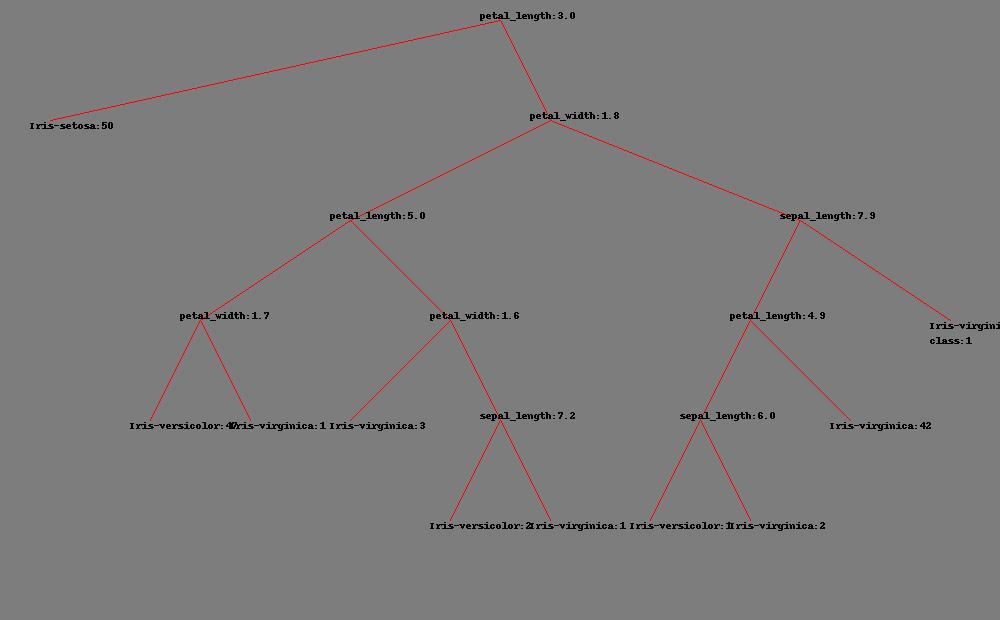
\includegraphics[max size={\textwidth}{\textheight}]{tree-iris}\\~\\
HABERMAN \\
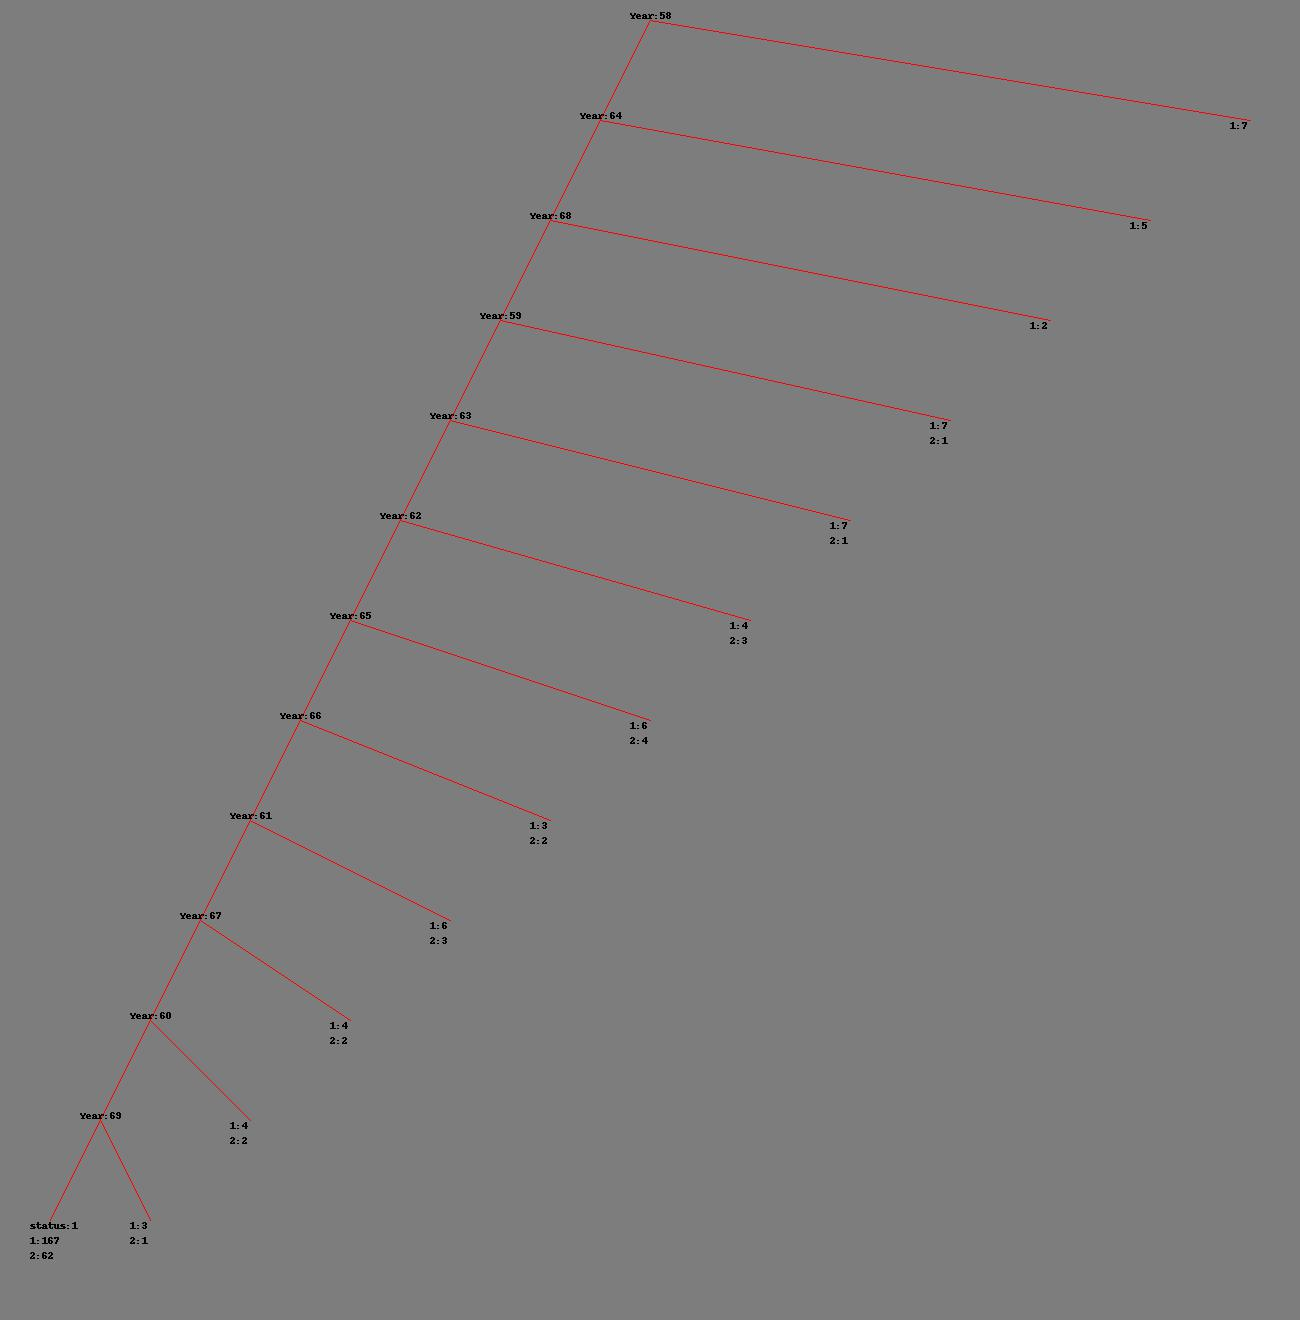
\includegraphics[max size={\textwidth}{\textheight}]{tree-haberman}\\~\\
WINE\\
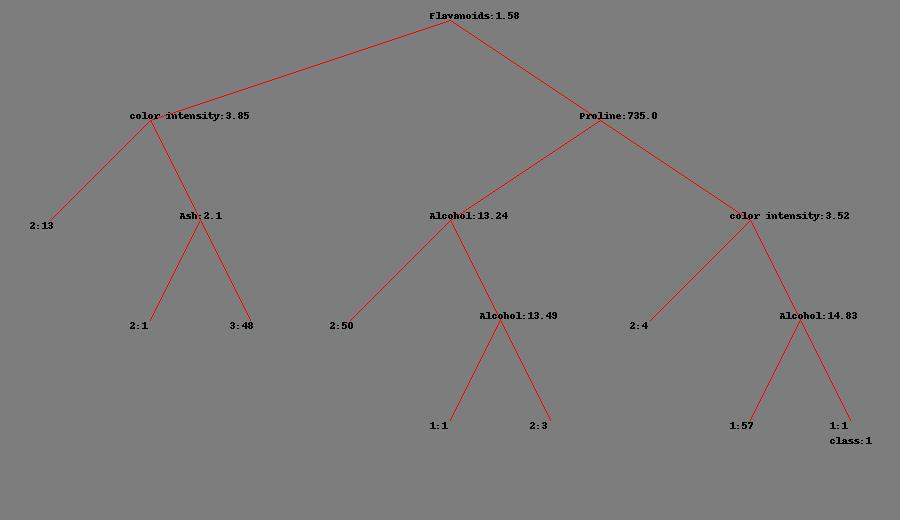
\includegraphics[max size={\textwidth}{\textheight}]{tree-wine}\\~\\
BANKNOTE
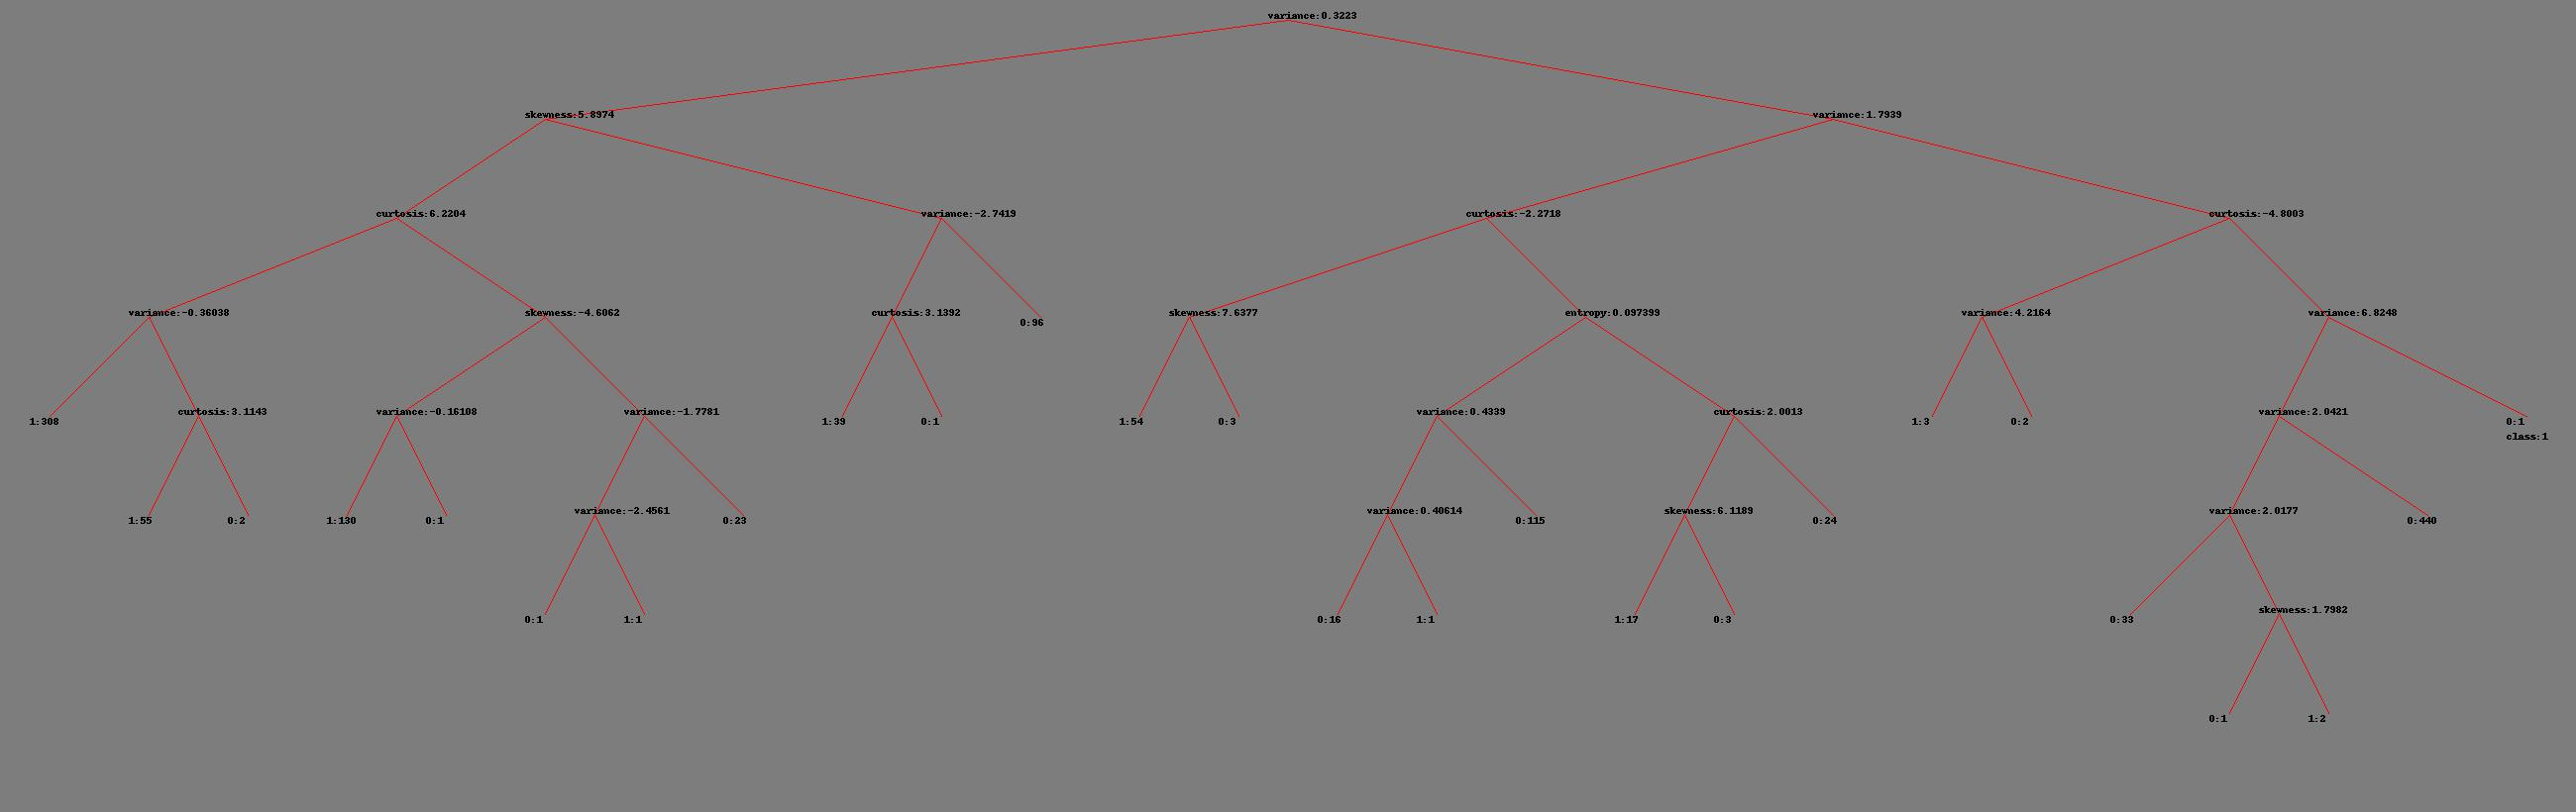
\includegraphics[max size={\textwidth}{\textheight}]{tree-banknote}\\~\\
}
\subsection{Section 3}{
Compare Gini and information gain as splitting criteria and discuss any observation on the
quality of splitting.\\~\\
1.) Gini to calculate gain is much faster as compared to Entropy since it avoids logs and lambda functions.\\
2.) Gini is used to work on Continuous Attributes contrary to the Entropy for classes.\\
3.) While Gini is used for minimising Misclassification whereas Entropy for Exploratory Data Analysis.\\
4.) There is hardly any difference while you use gini or entropy. (Approximately maximum of ~5%)\\~\\
}

}
\section{Question 5 Solution}{
Modify your decision tree from the previous question and evaluate the overfitting prevention methods listed below. All evaluation should be carried out using 10-fold cross-validation as implemented in the previous Problem, but the performance should be evaluated using multiple measures.\\~\\
\subsection{Section 1}{
Use pessimistic estimates of the generalization error by adding a penalty factor 0.5 for each node in the tree.\\~\\
1.) There are two methods which could have been chosen at this point Post and Pre Pruning, we go ahead with post pruning due to the computational limitations and code architecture limitations. Also, the pessimistic error is calculate on basis of over all training error and the number of training records keeping in mind the penalty applicable on each leaf node.\\~\\
Few of the Pruned Trees:\\~\\
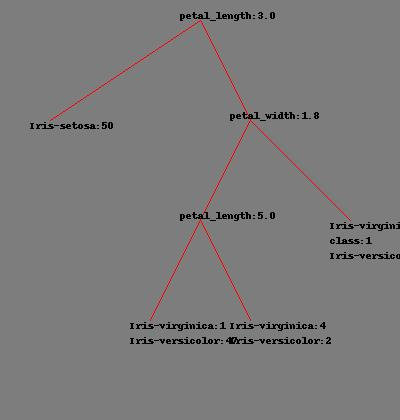
\includegraphics[max size={\textwidth}{\textheight}]{tree-prune-iris}\\~\\
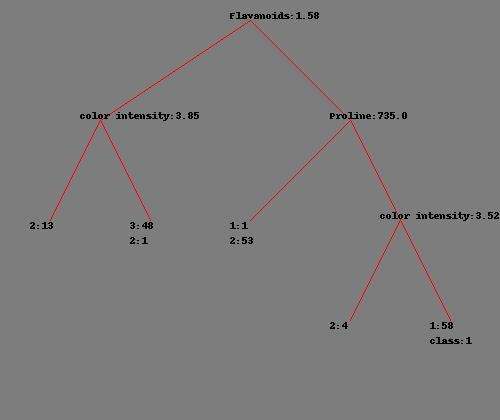
\includegraphics[max size={\textwidth}{\textheight}]{wine}\\~\\
}
\subsection{Section 2}{
Use a validation set that consists of 25\% of the training partition\\~\\
1.) The algorithm is splitting the already split data to consider that for validation set.\\
2.) It continues to follow the first question for the K Fold Stratified Sampling\\
3.) The validation test is used to test at each decision instance of the tree. As we start building the tree the issue I was stuck at was to maintain a node count. I just wanted to check the validation accuracy. In theory I should stop the tree growth as the validation set accuracy does not increment any more.\\~\\
}
\subsection{Section 3}{
Use the minimum description length principle, as explained in Question \#8, page 201 of
your Textbook.\\~\\
\centerline{MDL Formula:}~\\
\centerline{Cost(tree,data) = Cost(tree) + Cost(data/tree)}~\\

\[Cost of Encoding each Attribute = log_2(m)\]
\[Cost of Encoding each Class = log_2(k)\]
The basic logic is to find the difference between the parent and the child node as cost of encoding class and attribute is constant and we need to calculate the cost for the penalty incurred.\\~\\
}
}

\section{Question 6 Solution}{
Beyond greedy: combining beam search and classification tree construction. Extend the greedy algorithm for tree learning developed in the previous two questions to find a better classification tree as follows: At each step of node splitting, instead of picking the single best attribute to find the successor tree, keep top m successor trees based on the splits according to the top m attributes. For each of the trees in the list, generate the successor tree by splitting according to the next attribute. Then, keep top m successor trees (from all generated trees) for the next step and drop all the others. Continue the process until the stoppage criteria are fulfilled and select the best remaining tree as your model. Compare this algorithm with the greedy classification tree learning algorithm (m = 1) and comment on what you observe. Feel free to adjust this algorithm and experiment with different m’s and other parameters to see whether there is improvement in accuracy.\\~\\
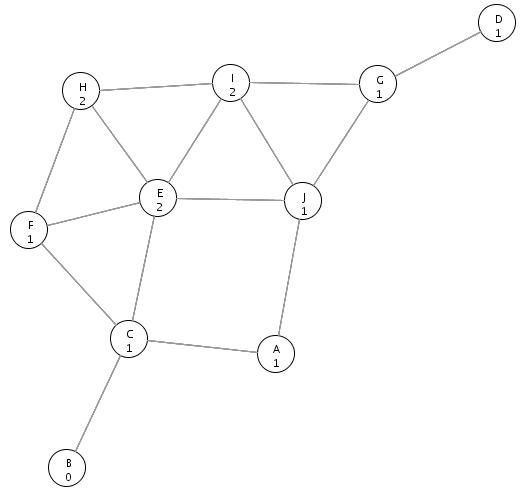
\includegraphics[max size={\textwidth}{\textheight}]{beam1}\\~\\

Here we implement the Beam Search Algorithm in combination with the Breadth First Search Tree. We need to maintain M trees and select the best resulting atributes from each tree. The worst case will be that the attributes will be spread over m trees while the best cases will be when all the best attributes will be found in one place.\\~\\


}
\section{References}{
Discussed with Krish Mahajan.
1.) https://www.quora.com/How-is-the-market-for-BI-tool-Tableau-What-is-its-future-Is-it-a-good-career-choice\\
2.) https://www.quora.com/Is-Tableau-good-from-a-career-point-of-view\\
3.) http://stats.stackexchange.com/questions/94886/what-is-the-relationship-between-the-gini-score-and-the-log-likelihood-ratio \\
4.) https://www.garysieling.com/blog/sklearn-gini-vs-entropy-criteria \\
}
\end{document}